\documentclass{tudelft-report}
\usepackage{biblatex}
\usepackage{float}
\addbibresource{report.bib}
\usepackage{amsthm}
\usepackage{thmtools}
\usepackage{tcolorbox}
\usepackage{tikz}
\usetikzlibrary{arrows,shapes,positioning,shadows,trees,mindmap}
\usepackage[edges]{forest}
\usetikzlibrary{arrows.meta}
\colorlet{linecol}{black!75}
\usepackage{xkcdcolors}
\usepackage{tikz}
\usetikzlibrary{backgrounds}
\usetikzlibrary{arrows,shapes}
\usetikzlibrary{tikzmark}
\usetikzlibrary{calc}
\newcommand{\highlight}[2]{\colorbox{#1!17}{$\displaystyle #2$}}
\newcommand{\highlightdark}[2]{\colorbox{#1!47}{$\displaystyle #2$}}
\renewcommand{\highlight}[2]{\colorbox{#1!17}{#2}}
\renewcommand{\highlightdark}[2]{\colorbox{#1!47}{#2}}
\newcommand{\lap}{\mathrm{Lap}}
\newcommand{\pr}{\mathrm{Pr}}

\newcommand{\Tset}{\mathcal{T}}
\newcommand{\Dset}{\mathcal{D}}
\newcommand{\Rbound}{\widetilde{\mathcal{R}}}

\setlist{itemsep=-2pt}
\renewcommand{\deg}{\si{\degree}\xspace}

\declaretheoremstyle[
spaceabove=6pt, spacebelow=6pt,
headfont=\normalfont\bfseries,
notefont=\mdseries, notebraces={:}{ },
bodyfont=\normalfont,
postheadspace=\newline
]{mystyle}
\declaretheorem[thmbox = M, name = Proposition,style=mystyle]{proposition}
\usepackage[super]{nth}
\begin{document}
\frontmatter
\title{Optimal allocation of bacterial resources
in a bioreactor}
\subtitle{Introduction to optimal control problems}
\author{Lélio Astruc \& Nathan Edery}

\subject{MAM4 : Project report}
\coverimage{figures/waa_auto_x2.jpg}
\definecolor{title}{HTML}{4884d6}
\makecover
\begin{titlepage}

\begin{center}
{\makeatletter
\largetitlestyle\fontsize{45}{45}\selectfont\@title
\makeatother}

{\makeatletter
\ifdefvoid{\@subtitle}{}{\bigskip\titlestyle\fontsize{20}{20}\selectfont\@subtitle}
\makeatother}

\bigskip
\bigskip

by

\bigskip
\bigskip

{\makeatletter
\largetitlestyle\fontsize{25}{25}\selectfont\@author
\makeatother}

\bigskip
\bigskip

\setlength\extrarowheight{2pt}


\vfill

\begin{tabular}{ll}
    Instructor : & Jean-Baptiste Caillau \\
    With the help of : & Agustín Gabriel Yabo \\
    Project Duration : & October, 2023 - December, 2023 \\
    Department : & Applied Mathematics and Modelling\\
    Cover : & DALL•E 3
\end{tabular}

\bigskip
\bigskip

\begin{tabular}{p{15mm}p{10cm}}
    %Cover: & DALL•E 3 \\
    % Feel free to remove the following attribution, it is not required - still appreciated :-)
\end{tabular}

\end{center}

%% Insert the TU Delft logo at the bottom of the page


\end{titlepage}

\chapter*{Preface}
\addcontentsline{toc}{chapter}{Preface}

\emph{\indent Studying tiny life forms using resource sharing models has been a game-changer in batch bioprocessing. It helps one understand how bacteria behave naturally by figuring out how they divide their resources through smart methods. \\ \\
\indent This report dives into batch bioprocessing but from a different angle, looking at how resources are used, since we are the one poking around in this model to see how things change over time and if they stay stable when controlling it through a mathematical theory. We have used a basic model for bacteria growth called the self-replicator model that considers what is happening inside the bioreactor. We have done numerical resolutions of $ODEs$ using Julia and tried helping Mr. Yabo in the completion of his work.\\ \\
\indent Solving complex mathematical problems were interesting as we faced several problems that taught us how real-worlds mathematical research is.}

\begin{flushright}
{\makeatletter\itshape
    \@author \\
    Biot, \monthname{} \the\year{}
\makeatother}
\end{flushright}

\tableofcontents

\mainmatter

\chapter{Introduction}
\label{chapter:introduction}
The exploration of microorganisms using resource allocation models has gained significance in understanding their behaviors via simplified dynamic models. This project illustrates how cellular resources are managed through optimal control theory. It's crucial for tackling various challenges, like optimizing metabolite production or final volume, while controlling bacterial growth, which has practical applications in industries like food preservation and biofuel production. \\ \\
This report focuses on batch bioprocessing from a resource allocation perspective, exploring different scenarios and focusing on the biomass maximisation case.\\ \\
Through this paper, we will discuss about maximizing a criterion through Optimal Control Theory and beginning in symbolic mathematics.
\chapter{Definition of the model}
\label{chapter:definition}
The fed-batch bioreactor considered in this work is represented below. The \verb|fed-batch reactor| contains the substrate $S$ at an initial volume $\mathcal{V}_e$, with a concentration of metabolites of interest $X$ and the volume of bacterial population $\mathcal{V}_i$. The inflow of \verb|F| produces an increase of the volume $\mathcal{V}_e$.
\begin{figure}[H]
    \centering
    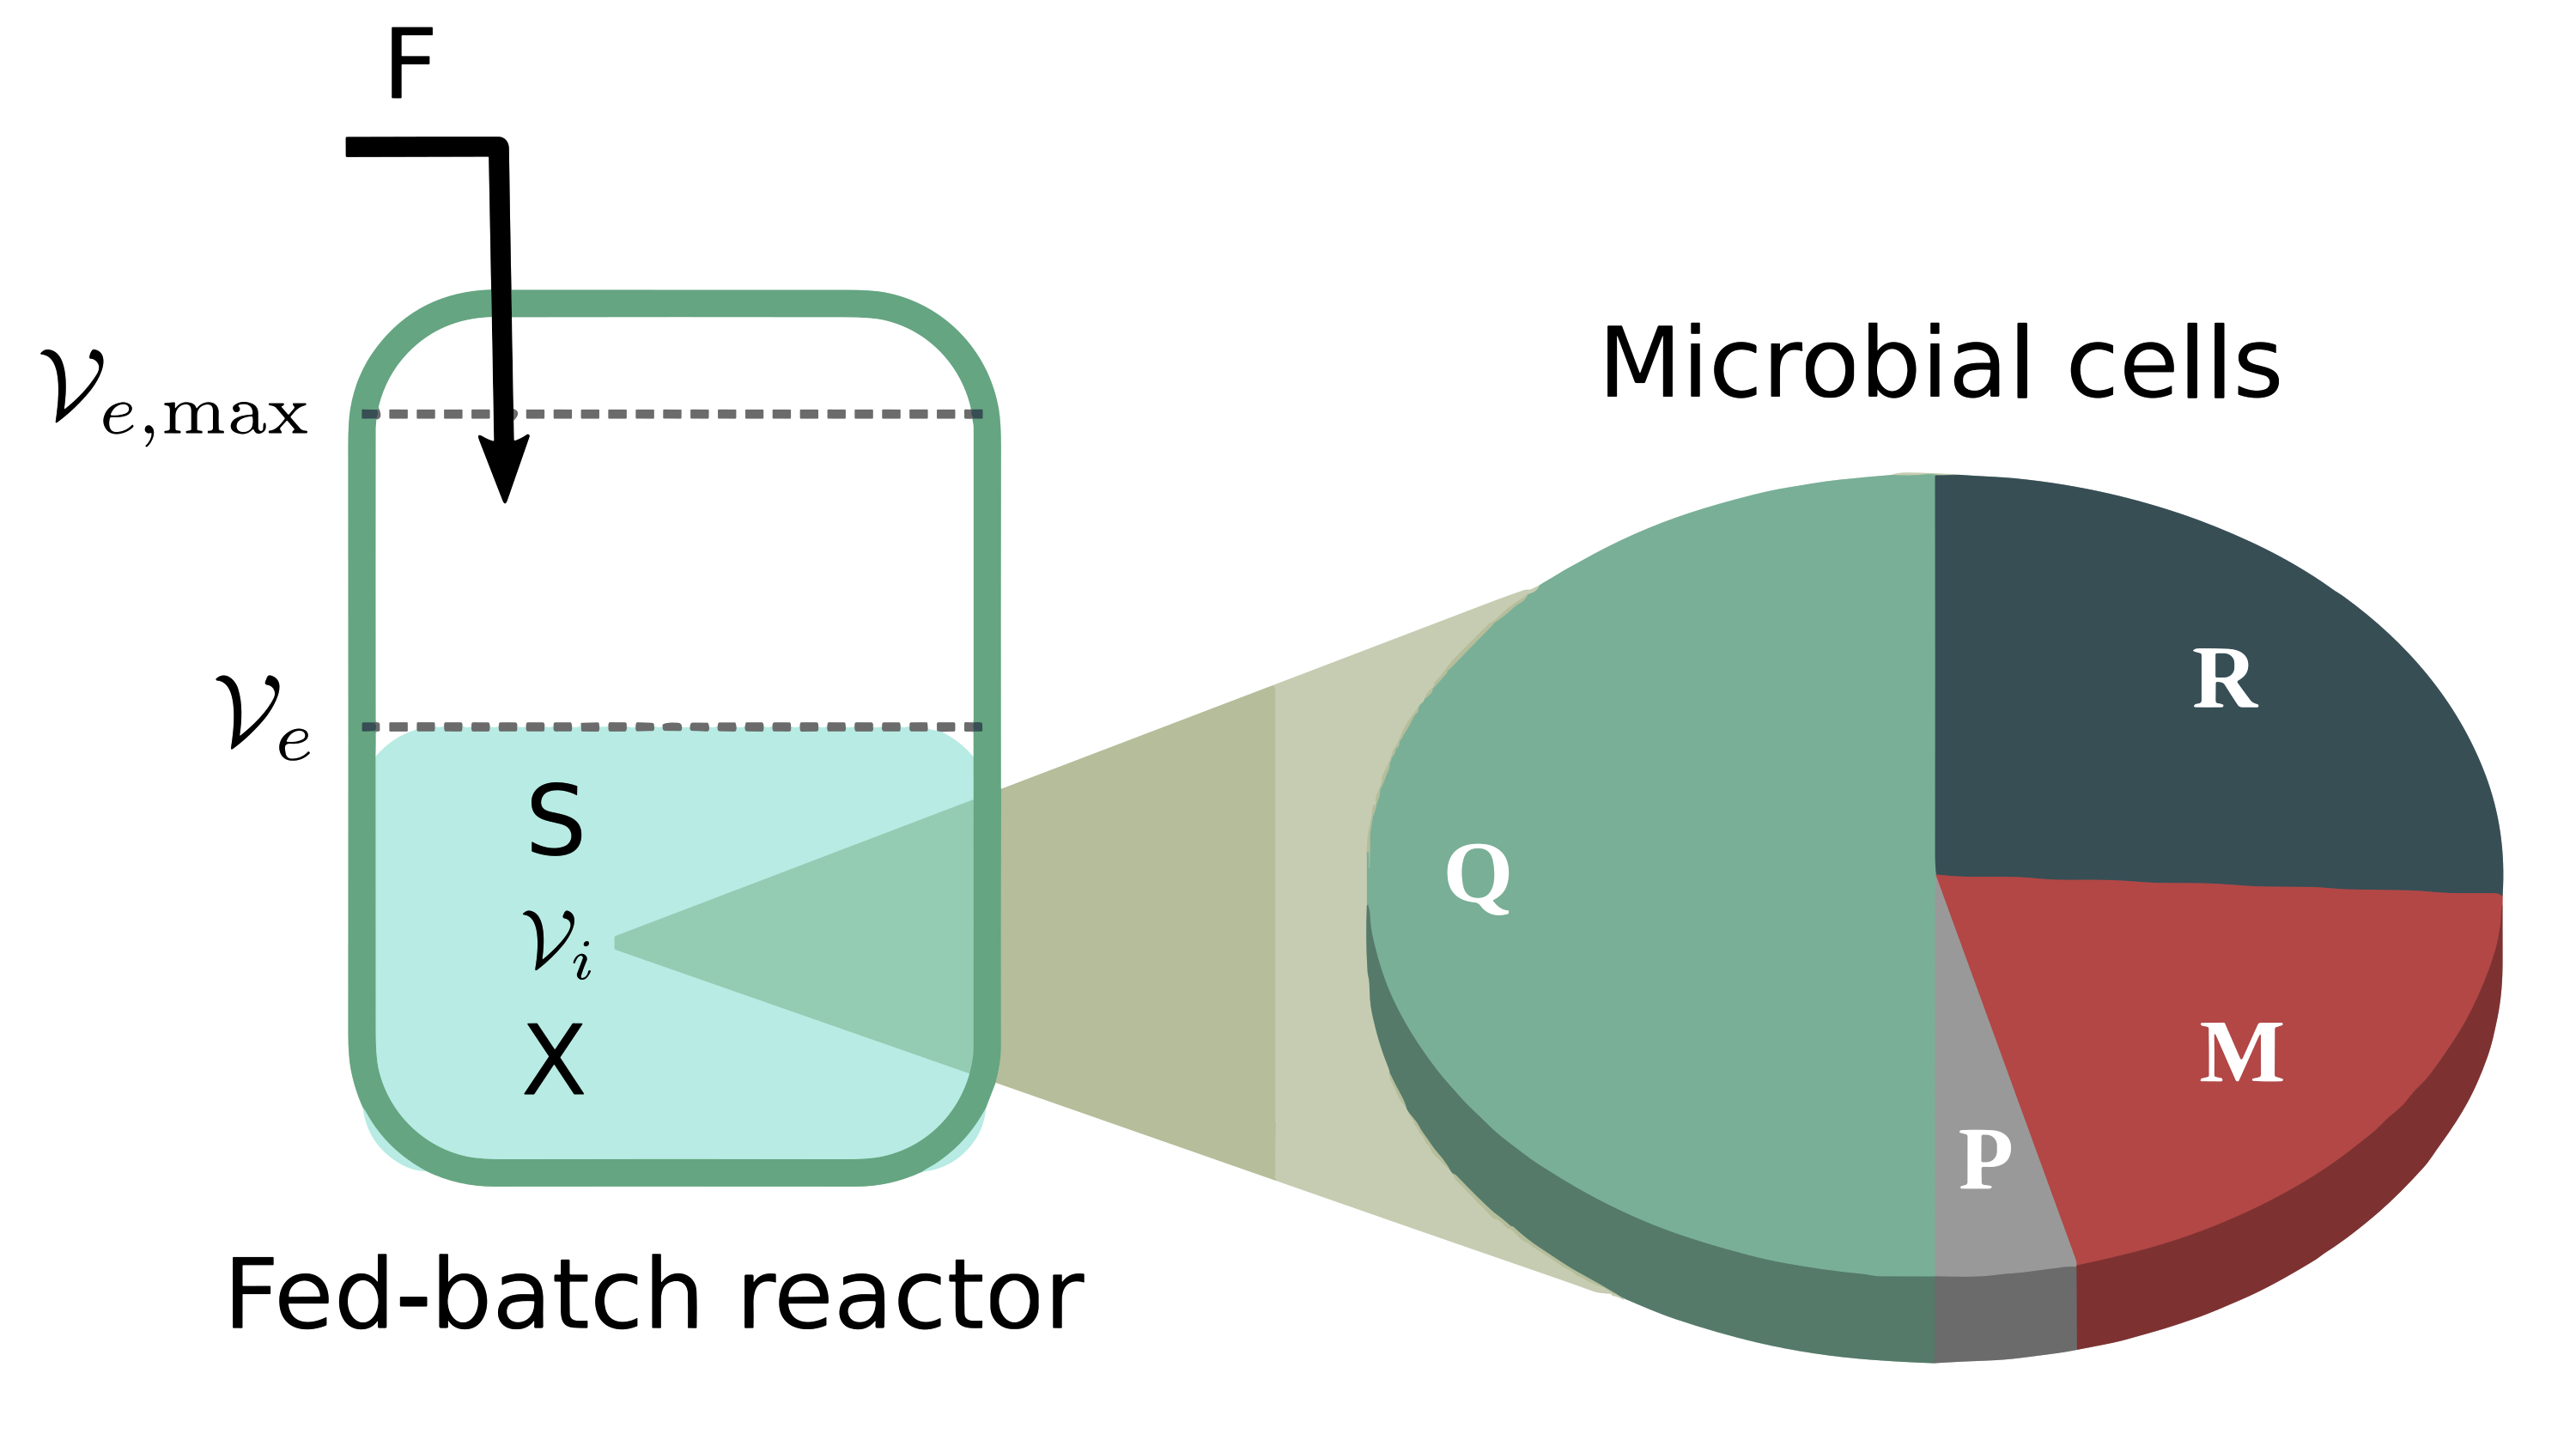
\includegraphics[scale = 0.3]{figures/bioreactorScheme.png}
    \caption*{The fed-batch reactor}
\end{figure}
\addcontentsline{toc}{section}{The self-replicator model}
\section*{The self-replicator model}\noindent
The self-replicator model illustrates the variation over time of a microbial population's caracteristics inside a bioreactor. We start with a constant volume $\mathcal{V}_e$ of microbial population and a certain mass $S$ of substrate that will be ``eaten'' by the microbial population to be transformed into precursor metabolites called $P$. Those precursors produce proteins that are of $3$ different types : $M$, $R$ and $Q$.\\
The class $M$ protein is responsible for the absorption of substrate $S$ and production of precursors $P$ and metabolites of interest called $X$.\\
The class $R$ protein is representing ribosomes, handling the production of proteins of class $M$, $R$ and $Q$.\\
The class $Q$ protein is independant of the growth rate represent the proteins maintaining the cell and the ribosomes.

\begin{figure}[H]
 \centering
 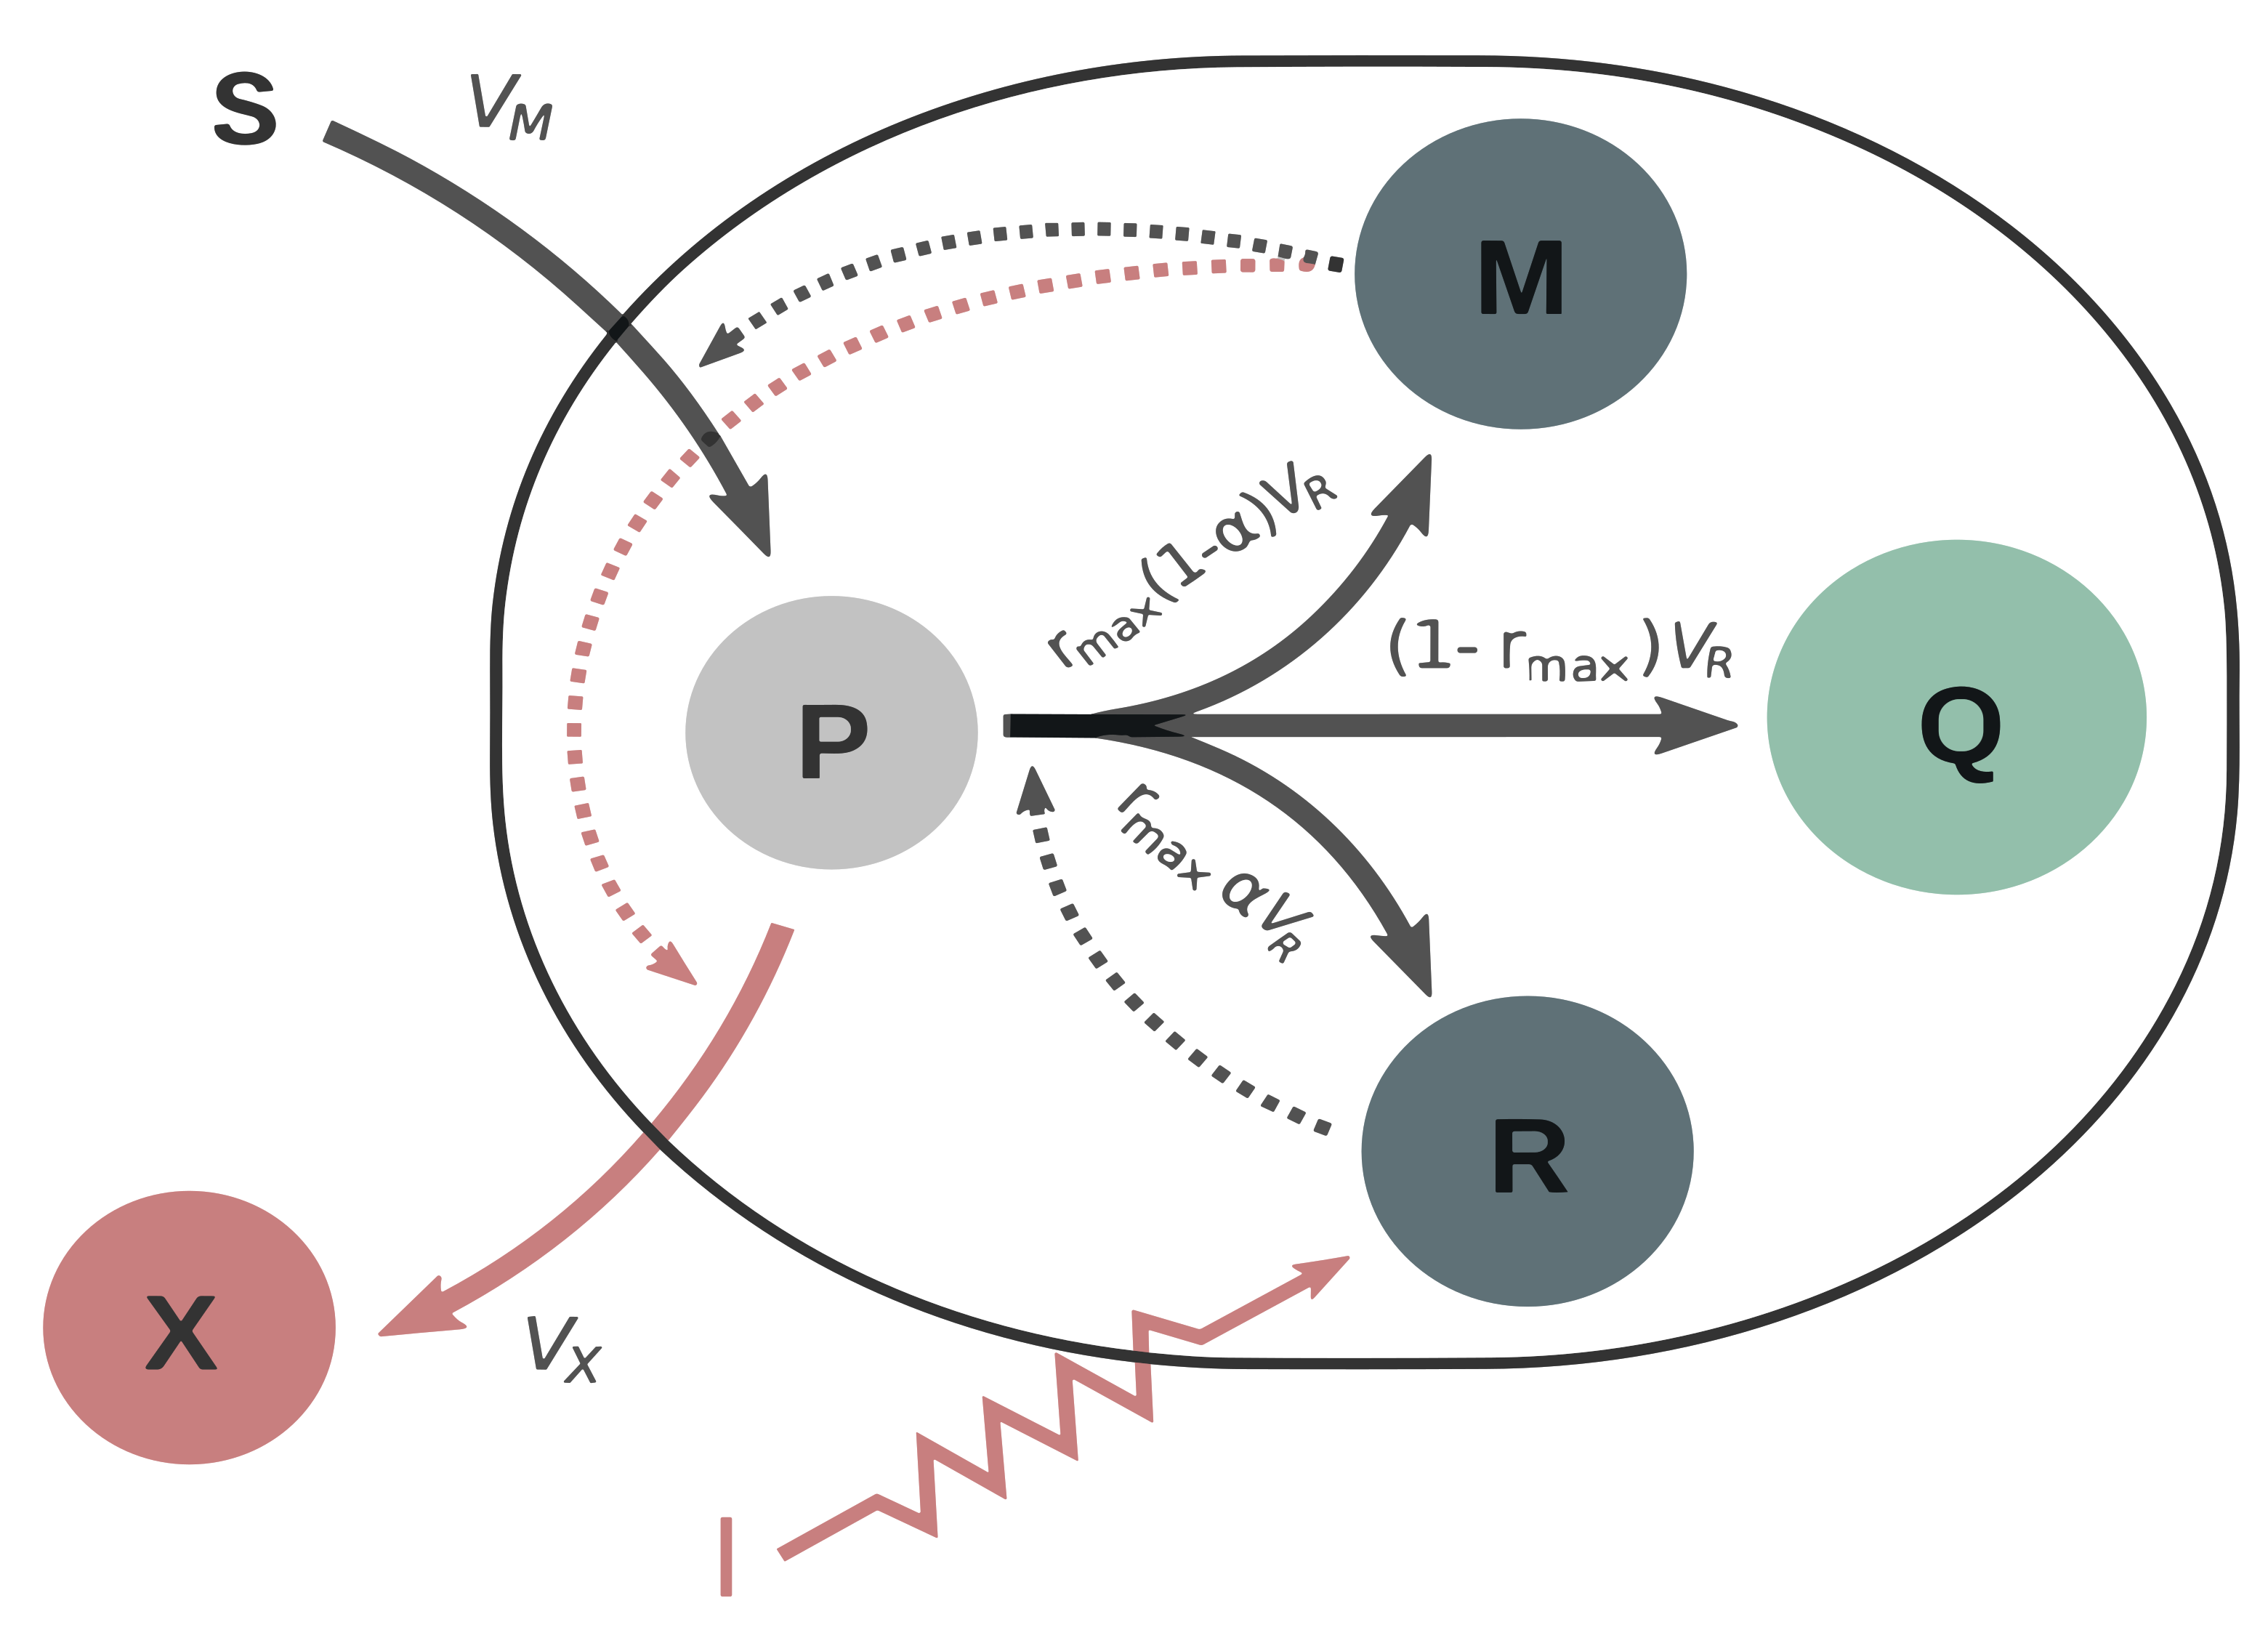
\includegraphics[scale=0.13]{figures/modele.png}
 \caption*{The self-replicator model}
\end{figure}\noindent
Solid arrows on the scheme represent a flow of resources while dashed arrows are a catalyzing effect, for example the production of proteins $M$, $R$ and $Q$ are all three catalyzed by the proteins of class $R$.\\ 
$V_R$ represents the synthesis rate of intercellular proteins measured in grams per hour. $r_{max}$ is an empirical constant that imposes a maximum to the rate of production of proteins $M$ and $R$. The growth-rate of $Q$ is in some way fixed whereas the balance between the one of $R$ and $M$ is decided by the control $\alpha$. We define $\alpha(t) \in [0,1]$ where $\alpha = 0$ means there will be no production of protein $R$ and $\alpha = 1$ means there will be no production of protein $M$.
\addcontentsline{toc}{section}{The dynamics of the self-replicator model}
\section*{The dynamics of the self-replicator model}\noindent
The dynamics of the self-replicator model are described by
\begin{equation*}\tag{SRM-D}\label{eq:srmd}
 \begin{cases}
  \dot{S} &= -V_M\\
  \dot{P} &= V_M - V_X - V_R\\
  \dot{R} &= r_{max}uV_r\\
  \dot{M} &= r_{max}(1-u)V_R\\
  \dot{Q} &= (1-r_{max})V_R\\
  \dot{X} &= V_X
 \end{cases}
\end{equation*}\noindent
$u(t)$ is the allocation control previously defined and we define the volume in liters of the microbial population $\mathcal{V}(t)$ as
$$\mathcal{V}\ \dot{=}\ \beta (M + R + Q)$$
where $\beta$ is some real constant.\\
Following this principle, we can define the concentration varying over time as 
$$p\ \dot{=}\ \frac{P}{\mathcal{V}} \quad\quad r\ \dot{=}\ \frac{R}{\mathcal{V}} \quad\quad m\ \dot{=}\ \frac{M}{\mathcal{V}} \quad\quad q\ \dot{=}\ \frac{Q}{\mathcal{V}}\quad\quad s\ \dot{=}\ \frac{S}{\mathcal{V}_e}\quad \quad x\ \dot{=}\ \frac{X}{\mathcal{V}_e}$$
We can also define 
$$v_M(s, m)\ \dot{=}\ \frac{V_M}{\mathcal{V}}\quad\quad v_R(p, r)\ \dot{=}\ \frac{V_R}{\mathcal{V}}$$
Supposing that these synthesis rate of ribosomes and precurors are linear in $m$, we can define 
$$v_M(s,m) = w_M(s)m\quad\quad v_R(p,r) = w_R(p)r$$
where $w_M(s)$ and $w_R(p)$ are \textit{Michaelis-Menten} kinetics functions defined as 
$$w_R(p)\ \dot{=}\ \frac{k_Rp}{K_R+p}\quad \textrm{ and }\quad w_M(s) \ \dot{=}\ \frac{k_Ms}{K_M+s}$$
\chapter{A glance at optimal control theory}
\label{chapter:ocp}
\indent Optimal control theory is a branch of mathematics and engineering that deals with finding the best control inputs to maximize or minimize a certain objective function, subject to a set of constraints. It's used in various fields, including engineering, economics, and biology, to determine the most efficient way to control a system.\\
\\
At its core, optimal control involves a few key components :
\begin{itemize}
 \item[$*$] \textbf{System dynamics }: this deals with how the system evolves over time. We usually represent it using $ODEs$.
 \item[$*$] \textbf{Control inputs }: these are the actions one can make to influence the modifications of the system. Optimizing a criterion means to find the best control input possible.
 \item[$*$] \textbf{Objective }: this is what we want to achieve (\emph{e.g.\ maximizing a money profit, minimizing energy consumption}).
\end{itemize}\noindent
The main idea behind optimal control is to find the control inputs that minimize or maximize the objective while considering system dynamics and any constraints imposed on the system. The solution typically involves calculus of variations, dynamic programming, \textit{Pontryagin}'s maximum principle, or numerical optimisation techniques.\\ \\
Optimal control theory has applications in various fields, such as robotics, aerospace engineering (like spacecraft trajectory optimisation), economics (such as optimal resource allocation), and even in designing optimal medical treatments.\\ \\
Here we use optimal control theory to maximize the volume $\mathcal{V}$ of the substrate.
\addcontentsline{toc}{section}{Formulation of an optimal control problem}
\section*{Formulation of an optimal control problem}\noindent
Let's consider the following problem, 
$$\begin{cases}
 \dot x = f(t,x,u)\\
 x(t_0) = x_0 & x_0,t \in \mathcal{I}
\end{cases}$$
where $\mathcal{I}$ is a compact interval of $\mathbb{R}$, $f$ is a continuous function from $\mathcal{I}\times\Omega\times U$ to $X$ where $X$ is a \textit{Banach} space. $\Omega$ is an open set of $X$ and $U$ a topological space. $U$ is generally $\mathbb{R}^n$.\\
The variable $x$ is the state and $u$ is the control. We assume that $x\longmapsto f(t,x,u)$ is differentiable for all $t$ and $u$.
$$J(u) = K(t_f,x_f) + \int_{t_0}^{t_f} \mathcal{L}(t,x(t), u(t))\,dt$$
where the lagrangian $\mathcal{L}$ satisfies the same conditions as $f$ and $K$ is differtiable on $\mathcal{V}_f$. $J(u$ is the performance criterion.
\addcontentsline{toc}{section}{A simple example of an optimal control problem}
\section*{A simple example of an optimal control problem}\noindent
Let's take the example of a plant growth. The caracteristics of a plant that we could optimize are numerous and we obviously can't take them all in consideration. Yet, we can take some of them. Let's consider the height of the plant ($h$), the thickness of its stem ($s$), the concentration of chlorophyll ($C$) and lastly the average length of its leaves ($\overline{l}$).\\
Let's say we want to maximize its height using a control $u$ being for example the light intensity over time. We model this as follows : \\\\
Let $u\in\mathbb{R}$, $x\in \mathbb{R}^4$, $t\in [t_0, t_f]$ and $x(t_0) = {}^t[h_0, s_0, C_0, \overline{l}_0]$
\begin{equation*}
\begin{cases}\tag{\ast}\label{eq:exempleocp}
   \dot x(t) = F_0(x(t)) + u(t)\cdot F_1(x(t))\\
   h(t_f) \longrightarrow max
  \end{cases}
\end{equation*}\noindent
Where $F_0(x)$ and $F_1(x)$ are vector fields that would take in consideration how the plant interacts with itself.\\ \\
We can solve this using numerical simulations that will give us the control $u$ that satisfies the optimisation problem.

\chapter{The biomass maximisation in a finite-time horizon}
\label{chapter:bm-ocp}
As we saw in chapter \ref{chapter:ocp}, optimal control theory is a really useful tool for optimizing a criterion. In our model, the states that could be maximized or minimized would be the concentration of substrate ($s$), concentration of precursor metabolites ($p$), concentration of ribosomes ($r$) and the volume ($\mathcal{V}$).\\
The values of these quantities are expressed in 
\begin{equation*}\Gamma = \left\{(s,\, p,\, r,\, \mathcal{V},\, x)\in\mathbb{R}^5 \mid s\geq 0,\, p\geq 0,\, 0\leq r\leq 1,\, \mathcal{V}\geq 0,\, x\geq 0 \right\}
\end{equation*}\noindent
 which allows us to set the initial conditions
\begin{equation*}\tag{IC}\label{eq:ic}
s(0) = s_0 >0,\, p(0) = p_0 >0,\, x(0) = 0, r(0) = r_0 \in (0,1),\, \mathcal{V}(0) = \mathcal{V}_0>0
\end{equation*}\noindent
\addcontentsline{toc}{section}{The biomass maximisation case}
\section*{The biomass maximisation case}\noindent
The following model fits both for an infinite time and a finite time horizon. We focused on doing the numerical simulations for the finite-time horizon. In the Wild-Type Bacteria Model \eqref{eq:wtbm} it is assumed that no metabolite is produced since it is not naturally produced and only artificially added.
\begin{equation*}\tag{WTB-M}\label{eq:wtbm}
\begin{cases}
 \dot{s} &= -w_M(s)(1-r)\mathcal{V}\\
 \dot{p} &= w_M(s)(1-r) - w_R(p) r  (p+1)\\
 \dot{r} &= (u-r) w_R(p) r\\
 \dot{\mathcal{V}} &= w_R(p) r  \mathcal{V}
\end{cases}
\end{equation*}\noindent
Now that the model is defined, we can define the optimal control problem to be solved :
\begin{equation*}\tag{BM-OCP}\label{eq:bmocp}
\begin{cases}
 \mathcal{V}(t_f) \longrightarrow max\\
 \textrm{using the dynamics of }\eqref{eq:wtbm}\\
 \textrm{using initial conditions }\eqref{eq:ic}\\
 u(\cdot)\in \mathcal{U}
\end{cases}
\end{equation*}\noindent
To numerically solve this $OCP$ we used the language \verb|Julia| that is really handful for mathematical computations as we will see in chapter \ref{chapter:liebrackets}. On top of that, our tutor's team at INRIA developped an interesting tool called \verb|control-toolbox|. Basically this \verb|Julia| package solves $OCP$ of our type as long as the problem is well defined. The code we used to solve this $OCP$ is available in section \ref{chapter:appendix}.
The simulations for an infinite time horizon being already made, we did the ones for a finite-time horizon and made sure the results were matching the ones found by Mr.Yabo. 

\begin{figure}[H]
    \centering
    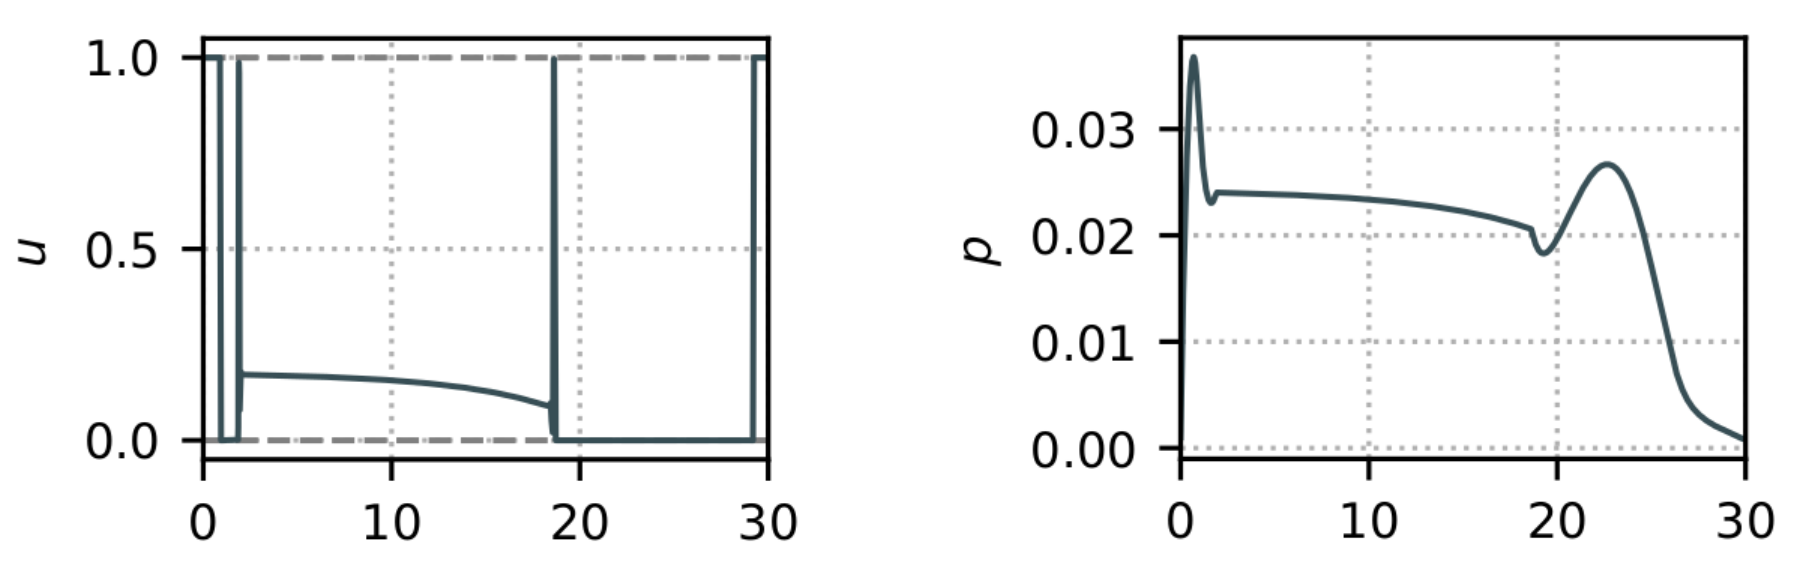
\includegraphics[width=\textwidth]{figures/control.png}
    \caption*{Numerical simulations of \eqref{eq:bmocp} with \eqref{eq:ic} $s_0 = 0.1,\, p_0 = 0.001,\, r_0=0.1,\, \mathcal{V}_0 = 0.003 $ and $t_f=30$.}
    \label{fig:control1}
\end{figure}
\begin{figure}[H]
\centering
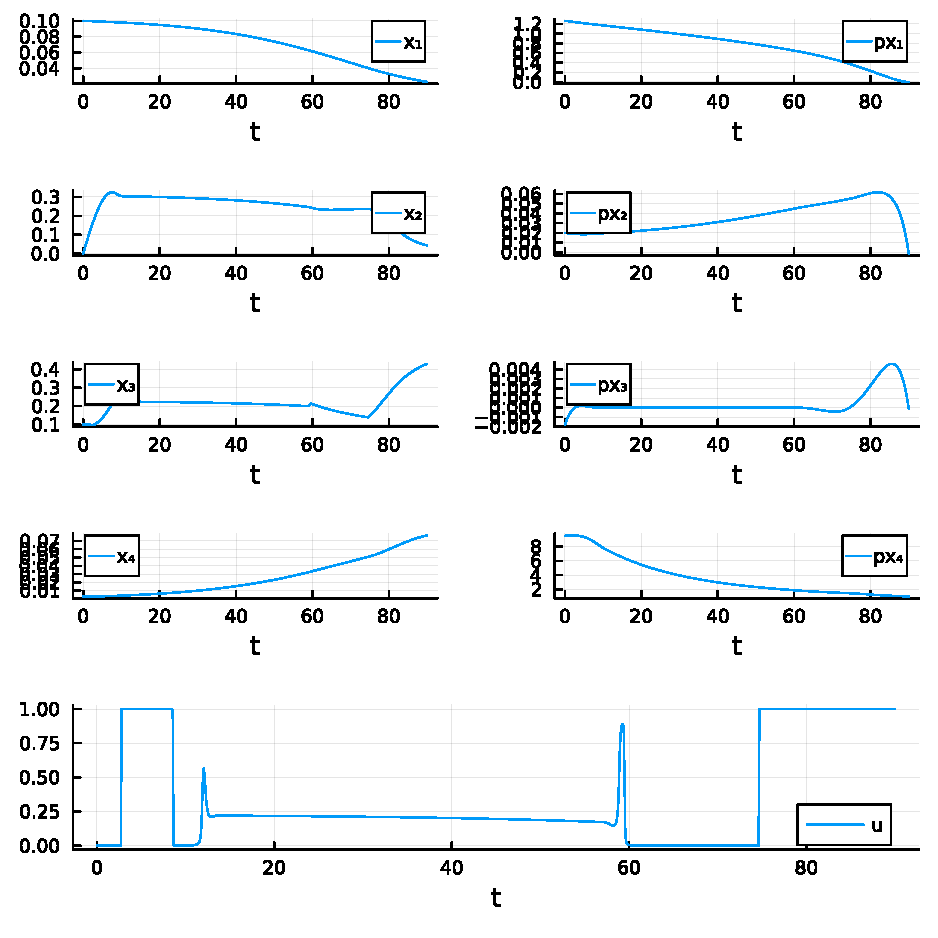
\includegraphics[width=\textwidth]{figures/tf_90.pdf}
\caption*{Our numerical solutions of \eqref{eq:bmocp} with \eqref{eq:ic} $s_0 = 0.1,\, p_0 = 0.001,\, r_0=0.1,\, \mathcal{V}_0 = 0.003 $ and $t_f=90$.}
\end{figure}
As we can see, the control $u$ is quite similar to the one Mr. Yabo found, and so is the graph of $p$ ($x_2$). Unfortunately, this is the case for a final time $t_f=90$, but not for $t_f=30$ as Mr. Yabo set. That problem is most likely due to the fact that the methods used in the \verb|OptimalControl| package are not the same as the ones used by Mr. Yabo used.
\chapter{Computing the \textit{Lie} brackets}
\label{chapter:liebrackets}
\addcontentsline{toc}{section}{What is a \textit{Lie} bracket}
\section*{What is a \textit{Lie} bracket}
On a vector space, a \textit{Lie} bracket is an internal composition law  on $V$ (meaning a \textit{Lie} bracket of two vectors is still a vector) that satisfies the following properties :
\begin{itemize}
 \item[$*$] \textbf{Bilinearity} : $\forall x, x', y \in V$, $\forall \lambda,\, \mu \in K$
 $$[\lambda x + \mu x', y] = \lambda[x, y] + \mu[x',y]$$
 \item[$*$] \textbf{Alternation} : $\forall x \in V$
 $$[x,x] = 0$$
 \item[$*$] \textbf{Jacobi's relation} : $\forall x,y,z\in V$ 
 $$[x,[y,z]] + [y,[z,x]] + [z,[x,y]] = 0$$
\end{itemize}
\addcontentsline{toc}{section}{Why did we use \textit{Lie} brackets}
\section*{Why did we use \textit{Lie} brackets}
In the preprint produced by Mr. Yabo and Mr. Caillau, a propostion was left to prove. Here it is
\color{title}
\begin{proposition}[Order of singular extremals]\color{black}\label{proposition:lie}\indent
 If the \textit{Lie} bracket $F_{101}$ belongs to the span of $F_1$ and $F_{01}$ , then
singular extremals must be of (local) order at least two.
\end{proposition}\color{black}\noindent
Since our problem is modelled as $$\dot{x}(t) = F_0(x(t)) + u\cdot F_1(x(t))$$
we proved this proposition using \textit{Lie} brackets with $F_{01} = [F_0, F_1]$ and $F_{101} = [F_1, F_{01}]$ and in our case ($V=\mathbb{R}^n$($n=4$)), \textit{Lie} brackets are defined as follows : 
$$[X, Y] = Y'X - X'Y$$ where $X,Y\in\mathbb{R}^n$ and $X'$ is the Jacobian of $X$ (same for $Y$).
\addcontentsline{toc}{section}{Computing \textit{Lie} brackets by hand}
\section*{Computing \textit{Lie} brackets by hand}
In \eqref{eq:bmocp}, we have vectors in $\mathbb{R}^4$, so the calculations of \textit{Lie} brackets imply hand-computing $4\times 4$ matrices determinants which can be quite tough (especially with non trivial functions). Even though this seemed hard, we gave it a try and quickly faced a wall : the matrices were not even fitting in landscape layout and we were pretty assured that we were leading to calculations error.
\addcontentsline{toc}{section}{Using symbolic mathematics}
\section*{Using symbolic mathematics}\noindent
Having in mind our problem was probably coming from the fact that some rational functions were not simplifying with each other, we thought it would probably be better if we used symbolic computation to do it for us.\\
That's why we used the \verb|Symbolics| package in \verb|Julia|. To prove the proposition, we adopted the following method : we calculated the \textit{Lie} brackets $F_{01}$ and $F_{101}$, then made sure that $rank(F_1, F_{01}) = rank(F_1, F_{01}, F_{101}) = 2$\\
We remember that 
$$F_0 = 
\begin{pmatrix}
 -w_m(s)(1-r)V \\
 w_m(s)(1-r)-w_r(p)r(1+p)\\
 -w_r(p) r^2\\
 w_r(p)rV
\end{pmatrix} \quad \textrm{ and } \quad F_1=
\begin{pmatrix}
 0\\ 
 0\\
 w_r(p)r\\
 0
\end{pmatrix}
$$
We then have, according to \verb|Symbolics| : $$F_{01} = 
\begin{pmatrix}
 \vspace{0.2cm}
 -\frac{p^2k_R^2rv}{(K_R + p)^2}\\
  \vspace{0.2cm}
 \frac{k_Rpr\big(\frac{k_Ms}{K_M+s}+\frac{k_Rp(1+p)}{K_R+p}\big)}{K_R+p} \\
  \vspace{0.2cm}
 \highlight{red}{$-\frac{r^2k_Rp\frac{k_Rp}{K_R+p}}{K_R+p} + \frac{2r^2p^2k_R^2}{(K_R+p)^2}$}+\bigg(\frac{k_Rr}{K_R+p} + \frac{-k_Rpr}{(K_R+p)^2}\bigg)\bigg(\frac{k_M(1-r)s}{K_M+s}+\frac{-k_Rp(1+p)r}{K_R+p} \bigg)\\
  \vspace{0.2cm}
 -\frac{p^2k_R^2rv}{(K_R+p)^2}
\end{pmatrix}
$$
which is easily reductible and almost disconcerting to note that such easy simplifications were not done by \verb|Symbolics| (\emph{e.g.\ the \highlight{red}{red-higlighted} bloc}).\\
Simplifications give us the following matrix $$F_{01} = 
\begin{pmatrix}
 \vspace{0.2cm}
 -\frac{p^2k_R^2rv}{(K_R + p)^2}\\
  \vspace{0.2cm}
 \frac{k_Rpr\big(\frac{k_Ms}{K_M+s}+\frac{k_Rp(1+p)}{K_R+p}\big)}{K_R+p} \\
 \vspace{0.2cm}
 \frac{r^2p^2k_R^2}{(K_R+p)^2} + \frac{k_RK_Rr}{(K_R+p)^2}\cdot \bigg(\frac{k_M(1-r)s}{K_M+s}+\frac{-k_Rp(1+p)r}{K_R+p} \bigg)\\
 -\frac{p^2k_R^2rv}{(K_R+p)^2}
\end{pmatrix}
$$
and same goes for $F_{101}$ which originally was :
$$F_{101} = 
\begin{pmatrix}
 \vspace{0.2cm}
 -\frac{p^3k_R^3rv}{(K_R+p)^3}\\
  \vspace{0.2cm}
 \frac{p^2k_R^2r\big(\frac{k_Ms}{K_M+s} + \frac{k_Rp(1+p)}{K_R+p}\big)}{(K_R+p)^2}\\
  \vspace{0.2cm}
 \alpha\\
  \vspace{0.2cm}
 -\frac{p^3k_R^3rv}{(K_R+p)^3}
\end{pmatrix}
$$ with $\alpha$ being so big that we have to define it apart from the matrix if we want to fit it in the page.
\begin{align*}
 \alpha = &-\frac{k_Rp\bigg(\frac{-r^2k_Rp\frac{k_Rp}{K_R+p}}{K_R+p} + \frac{2r^2p^2k_R^2}{(K_R+p)^2} + \big(\frac{k_Rp}{K_R+p}-\frac{k_Rpr}{(K_R+p)^2}\big)\big(\frac{k_M(1-r)s}{K_M+s}-\frac{k_Rp(1+p)r}{K_R+p}\big)\bigg)}{K_R+p} \\&+ \frac{k_Rpr\bigg(\frac{4p^2k_R^2r}{(K_R+p)^2}-\frac{2p^2k_R^2r}{(K_R+p)^2}-\big(\frac{k_Rr}{K_R+p}-\frac{k_rpr}{(K_r+p)^2}\big)\big(\frac{k_rp(1+p)}{K_R+p}+\frac{k_Ms}{K_M+s}\big)\bigg)}{K_R+p}
\end{align*}

But it easily becomes 
$$F_{101} = 
\begin{pmatrix}
 \vspace{0.2cm}
 -\frac{p^3k_R^3rv}{(K_R+p)^3}\\
  \vspace{0.2cm}
 \frac{p^2k_R^2r\big(\frac{k_Ms}{K_M+s} + \frac{k_Rp(1+p)}{K_R+p}\big)}{(K_R+p)^2}\\
  \vspace{0.2cm}
 \frac{3k_R^3p^3r^2}{(K_R+p)^3}-\frac{k_R^2K_Rp^2r(1-r)^2}{(K_R+p)^3}\bigg(\frac{k_Msr}{K_M+s}+\frac{k_Rp(1+p)(1+r)}{K_R+p}\bigg)-2\frac{k_R^2r^2pK_R}{(K_R+p)^3}\bigg(\frac{k_rp(1+p)}{K_R+p}+\frac{k_Ms}{K_M+s}\bigg) \\
  \vspace{0.2cm}
 -\frac{p^3k_R^3rv}{(K_R+p)^3}
\end{pmatrix}
$$
In a first time, to prove that $rank(F_1, F_{01}) = 2$ we just had to make sure that at least one determinants of the minor matrices was not null.\\
That part was quite easy using \verb|Symbolics| since we can use the \verb|Symbolics.det()| function, hence just having to make sure at least one of the determinants was not null. Here are the determinants we obtained : 
$$0$$
$$\frac{k_R^3p^3r^2v}{(K_R+p)^3}$$
$$0 $$
$$ \frac{k_R^2p^2r^2\big(\frac{-k_Rp(1+p)}{K_R+p} - \frac{k_Ms}{K_M+s}\big)}{(K_R+p)^2}$$ 
$$ 0$$
$$ -\frac{k_R^3p^3r^2v}{(K_R+p)^3}$$ 
We obviously see that at least one determinant is not null (\emph{see \eqref{eq:ic}}). \\
\\
Then, to still have a rank of $2$ when adding $F_{101}$, we need to make sure that all the determinants of the minors of $(F_1\ F_{01}\ F_{101})$ are this time null (else rank would be $3$). \\
Here are the determinants of the minors of the matrices : 
$$-\frac{p^2k_R^2rv\frac{-r^2p^3k_R^3\big(\frac{-k_Rp(1+p)}{K_R+p}-\frac{k_Ms}{K_M+s}\big)}{(K_R+p)^3}}{(K_R+p)^2} + \frac{p^3k_R^3rv\frac{-k_Rpr\frac{k_Rpr\big(\frac{-k_Rp(1+p)}{K_R+p}-\frac{k_Ms}{K_M+s}\big)}{K_R+p}}{K_R+p}}{(K_R+p)^3}$$ 
$$ 0$$
$$ \frac{r^2p^4k_R^4v\frac{p^2k_R^2rv}{(K_R+p)^2}}{(K_R+p)^4} - \frac{v^2r^3p^6k_R^6}{(K_R+p)^6}$$
$$ -\frac{r^3p^5k_R^5v\big(\frac{-k_Rp(1+p)}{K_R+p}-\frac{k_Ms}{K_M+s}\big)}{(K_R+p)^5} + \frac{r^2p^3k_R^3\frac{p^2k_R^2rv}{(K_R+p)^2}\big(-\frac{k_Rp(1+p)}{K_R+p} - \frac{k_Ms}{K_M+s}\big)}{(K_R+p)^3}$$
\verb|Symbolics| really has trouble simplfying, yet it is quite obvious that all the determinants are equal to $0$.\\
To sum up what we did ; \\
$rank(F_1\ F_{01}) = 2$ is proved, so is $rank(F_1\ F_{01}\ F_{101}) = 2$.\\
That means propostion \ref{proposition:lie} is proved.\\
We continued our research further and tried to see if this property was verified for any $w_M(s)$ and $w_R(p)$. The numerical results show that it is true and here are the proofs.\\
The matrices $F_{0}$ and $F_1$ are the following
$$ 
F_0=\begin{pmatrix}
 -(1-r)vw_M(s)\\
 (1-r)w_M(s) - (1+p)rw_R(p)\\
 -r^2w_R(p)\\
 rvw_R(p)
\end{pmatrix} \quad \quad \quad F_1 = 
\begin{pmatrix}
 0\\
 0\\
 rw_R(p)\\
 0
\end{pmatrix} $$ which give us the matrices $F_{01}$ and $F_{101}$ :
$$F_{01} =
\begin{pmatrix}
 -rvw_R(p)w_M(s)\\
 -(-w_M(s)+ (-1-p)w_R(p))rw_R(p)\\
 (w_R(p))^2r^2 + ((1-r)w_M(s)- (1+p)rw_R(p))r\frac{dw_R(p)}{dp}\\
 -(w_R(p))^2rv
\end{pmatrix}
$$
$$F_{101} =
\begin{pmatrix}
 -(w_R(p))^2rvw_M(s)\\
 (w_R(p))^2(w_M(s) - (-1-p)w_R(p))r\\
 \beta\\
 -(w_R(p))^3rv
\end{pmatrix}
$$
Where 
\begin{align*}
 \beta &= -\bigg((w_R(p))^2r^2 + ((1-r)w_M(s) - (1+p)rw_R(p))r\frac{dw_R(p)}{dp}\bigg)w_R(p) + \bigg(2(w_R(p))^2r \\
 &+ ((1-r)w_M(s) + (-1-p)rw_R(p))\frac{dw_R(p)}{dp}+ (-w_M(s) + (-1-p) w_R(p))r\frac{dw_R(p)}{dp}\bigg)rw_R(p) \\
 &+ r^2(-w_M(s) + (-1-p)w_R(p))w_R(p)\frac{dw_R(p)}{dp}
\end{align*}
Computing the determinants of the matrix $(F_1,\, F_{01})$ gives us the following results 
$$0$$
$$(w_R(p))^2r^2vw_M(s)$$
$$0$$
$$(w_R(p))^2r^2(-w_M(s)+(1-p)w_R(p)$$
$$0$$
$$-(w_R(p))^3r^2v$$
which clearly shows that at least one of them is not null (\emph{see} \eqref{eq:ic}).\\
\noindent
In the end we compute the determinants of the matrix $(F_1,\, F_{01},\, F_{101})$ to find that they all are equal to $0$ :
$$
 -(w_R(p))^4r^3(w_M(s)-(-1-p)w_R(p))vw_M(s)-(w_R(p))^4r^3(-w_M(s)+(-1-p)w_R(p))vw_M(s)$$
 $$0$$
 $$0$$
 $$-(w_R(p))^5r^3(-w_M(s)+(-1-p)w_R(p))v-(w_R(p))^5r^3(w_M(s)-(-1-p)w_R(p))v    $$
As above in the case of defined functions, \verb|Symbolics| has trouble simplfying, yet it is again quite easy to verify that they all are equal to $0$.\\
These results prove that the proposition  \eqref{proposition:lie} is true for any function $w_R(p)$ and $w_M(s)$.

\chapter{Conclusion}
\label{chapter:conclusion}
This three-month duration project helped us understanding many things in the world of scientific research.\\
Firstly that sometimes, calculations by hand can be really hard thus leading to miscalculations. We discovered symbolic mathematics through the language \verb|Julia| that we also discovered.\\
Secondly that a problem that might seem insignificant from a mathematical point of view, actually hides quite complex mathematics such as \textit{Lagrangian} and \textit{Hamiltonian} operations that we were not able to fully understand being in \nth{4} year. Yet, without a fullfill understanding of the mathematics behind the model, we were still able to fill the tasks we were assigned.\\
Finally, we enjoyed being in trouble while trying to complete this work and still finding a solution in the end.\\
We are happy to have chosen this subject and to have discovered things like optimal control theory and the language \verb|Julia|. We are especially thankful to Mr. Caillau and Mr. Yabo for helping us through this work and really enjoyed working with them.
%%%%%%%%%%%%%%%%%%%%%%%%%%%%%%%%%%%%%%%%%%%%%%%%%%%%%%%%%%%%%%%%%%%%%%%%%%%%%%%%%%%%%%%%%%%%%%%%%%%%%%%%%%%%%%%%%%%%%%%%%%%%%%%%%%%%%%%%%%%%%%%%%%%
 \setcounter{biburlnumpenalty}{7000}
 \setcounter{biburllcpenalty}{7000}
 \setcounter{biburlucpenalty}{7000}
 \printbibliography[heading=bibintoc,title=References]
\appendix
\chapter{Appendix}
\label{chapter:appendix}
Here is the code we used to do the calculations on the \textit{Lie} brackets and to solve the $OCP$ in a finite-time horizon. The code does not exactly use the same syntax since symbols encoded in \verb|utf-8| that are permitted in \verb|Julia| are not allowed in the environment \verb|lstlisting|. Hence, code like \verb|t in [ t0, tf ], time| actually uses $\in$ instead of plain-text ``in''.

\begin{lstlisting}
 """This is the code 
 for the ocp problem in 
 a finite time horizon"""
 using OptimalControl
 
 t0 = `0`         # initial time
 tf = `90`        # final time
 s0 = `0.1`       # initial substrate
 p0 = `0.001`     # initial precursors
 r0 = `0.1`       # initial ribosomes
 V0 = `0.003`     # initial volume

 G@defG ocp begin # definition of the optimal control problem

    t in [ t0, tf ], time
    x in R^4, state 
    u in R, control

    s = x_1
    p = x_2
    r = x_3
    v = x_4

    GxG(t0A)A == [ s0, p0, r0, V0 ]
    
    GsG(tA)A >= `0`
    GpG(tA)A >= `0`
    `0` <= GrG(tA)A <= `1`
    GvG(tA)A >= `0`
    `0` <= GuG(tA)A <= `1`

    Gdot_xG(tA)A == GF0G(x(t)A)A + GuG(tA)A * GF1G(x(t)A)A

    GvG(tfA)A -> max

 end;

 # Dynamics
 BconstB k_r = `1.1`
 BconstB k_m = `1.2`
 BconstB K_r = `1.3`
 BconstB K_m = `1.4`


 Gw_rG(pA)A = k_r * p / (K_r + pA)A
 Gw_mG(sA)A = k_m * s / (K_m + sA)A

 F0 = GVectorFieldG( phi -> begin
    s, p, r, V = phi
    return [ -Gw_mG(sA)A * (`1` - rA)A * V
              Gw_mG(sA)A * (`1` - rA)A - Gw_rG(pA)A * r * (p + `1`A)A
             -Gw_rG(pA)A * r^`2`
              Gw_rG(pA)A * r * V ]
 end A)A

 F1 = GVectorFieldG( phi -> begin
    s, p, r, V = phi
    return [ `0`, `0`, Gw_rG(pA)A * r, `0` ]
 end A)A

 direct_sol1 = GsolveG(ocp, grid_size=`100`A)A

 direct_sol2 = GsolveG(ocp, grid_size=`1000`A)A

 plt1 = GplotG(direct_sol1, size=(`600`, `600`)A)A
 plt2 = GplotG(direct_sol2, size=(`600`, `600`)A)A

\end{lstlisting}

\begin{lstlisting}
 """Symbolic computation of Lie brackets
 for 4x4 matrices determinants"""
 using Symbolics

 G@variablesG s, p, r, v
 G@variablesG w_m(s), w_r(p)
 

 F0 = [-w_m * (1-r)*v, w_m*(1-r) - w_r *r * (p+1), -w_r*r^2, w_r*r*v]
 F1 = [`0`, `0`, w_r*r, `0`]
 
 # Calcul du crochet de Lie de F0 et F1

 F0_prime = Symbolics.GjacobianG(F0, [s, p, r, v]A)A
 F1_prime = Symbolics.GjacobianG(F1, [s, p, r, v]A)A

 F01 = F1_prime * F0 - F0_prime * F1

 # Calcul du crochet de Lie de F1 et F01

 F01_prime = Symbolics.GjacobianG(F01, [s, p, r, v])

 F101 = F01_prime * F1 - F1_prime * F01
 
 # Calcul du rang de la matrice F1 et F01 :
 mat_F1_F01 = [F1 F01]
 
 # Sous matrice de mat_F1_F01
 sousDet1_F1_F01 = [mat_F1_F01[1] mat_F1_F01[5] ; mat_F1_F01[2] mat_F1_F01[6]]
 sousDet2_F1_F01 = [mat_F1_F01[1] mat_F1_F01[5] ; mat_F1_F01[3] mat_F1_F01[7]]
 sousDet3_F1_F01 = [mat_F1_F01[1] mat_F1_F01[5] ; mat_F1_F01[4] mat_F1_F01[8]]
 sousDet4_F1_F01 = [mat_F1_F01[2] mat_F1_F01[6] ; mat_F1_F01[3] mat_F1_F01[7]]
 sousDet5_F1_F01 = [mat_F1_F01[2] mat_F1_F01[6] ; mat_F1_F01[4] mat_F1_F01[8]]
 sousDet6_F1_F01 = [mat_F1_F01[3] mat_F1_F01[7] ; mat_F1_F01[4] mat_F1_F01[8]]
 
 mineur1_F1_F01 = Symbolics.GdetG(sousDet1_F1_F01A)A
 mineur2_F1_F01 = Symbolics.GdetG(sousDet2_F1_F01A)A
 mineur3_F1_F01 = Symbolics.GdetG(sousDet3_F1_F01A)A
 mineur4_F1_F01 = Symbolics.GdetG(sousDet4_F1_F01A)A
 mineur5_F1_F01 = Symbolics.GdetG(sousDet5_F1_F01A)A
 mineur6_F1_F01 = Symbolics.GdetG(sousDet6_F1_F01A)A
 
 # Calcul du rang de la matrice F1 F01 et F101
 mat_F1_F01_F101 = [F1 F01 F101]
 
 # Sous matrice de mat2
 sousDet1_F1_F01_F101 = [mat_F1_F01_F101[1] mat_F1_F01_F101[5] mat_F1_F01_F101[9] ;
 mat_F1_F01_F101[2] mat_F1_F01_F101[6] mat_F1_F01_F101[10] ; mat_F1_F01_F101[3]
 mat_F1_F01_F101[7] mat_F1_F01_F101[11]]

 sousDet2_F1_F01_F101 = [mat_F1_F01_F101[1] mat_F1_F01_F101[5] mat_F1_F01_F101[9] ;
 mat_F1_F01_F101[2] mat_F1_F01_F101[6] mat_F1_F01_F101[10] ; mat_F1_F01_F101[4]
 mat_F1_F01_F101[8] mat_F1_F01_F101[12]]
 
 sousDet3_F1_F01_F101 = [mat_F1_F01_F101[1] mat_F1_F01_F101[5] mat_F1_F01_F101[9] ;
 mat_F1_F01_F101[3] mat_F1_F01_F101[7] mat_F1_F01_F101[11] ; mat_F1_F01_F101[4]
 mat_F1_F01_F101[8] mat_F1_F01_F101[12]]

 sousDet4_F1_F01_F101 = [mat_F1_F01_F101[2] mat_F1_F01_F101[6] mat_F1_F01_F101[10] ;
 mat_F1_F01_F101[3] mat_F1_F01_F101[7] mat_F1_F01_F101[11] ; mat_F1_F01_F101[4]
 mat_F1_F01_F101[8] mat_F1_F01_F101[12]]
 
 mineur1_F1_F01_F101 = Symbolics.GdetG(sousDet1_F1_F01_F101A)A
 mineur2_F1_F01_F101 = Symbolics.GdetG(sousDet2_F1_F01_F101A)A
 mineur3_F1_F01_F101 = Symbolics.GdetG(sousDet3_F1_F01_F101A)A
 mineur4_F1_F01_F101 = Symbolics.GdetG(sousDet4_F1_F01_F101A)A
\end{lstlisting}
\begin{lstlisting}
 using Symbolics

 G@variablesG s, p, r, v
 G@variablesG w_m(s), w_r(p)

 F0 = [-w_m * (1-r)*v, w_m*(1-r) - w_r *r * (p+1), -w_r*r^2, w_r*r*v]
 F1 = [0, 0, w_r*r, 0]
 
 F0_prime = Symbolics.GjacobianG(F0, [s, p, r, v])
 F1_prime = Symbolics.GjacobianG(F1, [s, p, r, v])
 F01 = F1_prime * F0 - F0_prime * F1
 
 F01_prime = Symbolics.GjacobianG(F01, [s, p, r, v])
 F101 = F01_prime * F1 - F1_prime * F01
 
 mat_F1_F01 = [F1 F01]
 sousDet1_F1_F01 = [mat_F1_F01[1] mat_F1_F01[5] ; mat_F1_F01[2] mat_F1_F01[6]]

 sousDet2_F1_F01 = [mat_F1_F01[1] mat_F1_F01[5] ; mat_F1_F01[3] mat_F1_F01[7]]

 sousDet3_F1_F01 = [mat_F1_F01[1] mat_F1_F01[5] ; mat_F1_F01[4] mat_F1_F01[8]]

 sousDet4_F1_F01 = [mat_F1_F01[2] mat_F1_F01[6] ; mat_F1_F01[3] mat_F1_F01[7]]

 sousDet5_F1_F01 = [mat_F1_F01[2] mat_F1_F01[6] ; mat_F1_F01[4] mat_F1_F01[8]]

 sousDet6_F1_F01 = [mat_F1_F01[3] mat_F1_F01[7] ; mat_F1_F01[4] mat_F1_F01[8]]
 
 mineur1_F1_F01 = Symbolics.GdetG(sousDet1_F1_F01)
 mineur2_F1_F01 = Symbolics.GdetG(sousDet2_F1_F01)
 mineur3_F1_F01 = Symbolics.GdetG(sousDet3_F1_F01)
 mineur4_F1_F01 = Symbolics.GdetG(sousDet4_F1_F01)
 mineur5_F1_F01 = Symbolics.GdetG(sousDet5_F1_F01)
 mineur6_F1_F01 = Symbolics.GdetG(sousDet6_F1_F01)
 
 mat_F1_F01_F101 = [F1 F01 F101]
 
 sousDet1_F1_F01_F101 = [mat_F1_F01_F101[1] mat_F1_F01_F101[5] mat_F1_F01_F101[9] ;
 mat_F1_F01_F101[2] mat_F1_F01_F101[6] mat_F1_F01_F101[10] ; mat_F1_F01_F101[3]
 mat_F1_F01_F101[7] mat_F1_F01_F101[11]]

 sousDet2_F1_F01_F101 = [mat_F1_F01_F101[1] mat_F1_F01_F101[5] mat_F1_F01_F101[9] ;
 mat_F1_F01_F101[2] mat_F1_F01_F101[6] mat_F1_F01_F101[10] ; mat_F1_F01_F101[4]
 mat_F1_F01_F101[8] mat_F1_F01_F101[12]]

 sousDet3_F1_F01_F101 = [mat_F1_F01_F101[1] mat_F1_F01_F101[5] mat_F1_F01_F101[9] ;
 mat_F1_F01_F101[3] mat_F1_F01_F101[7] mat_F1_F01_F101[11] ; mat_F1_F01_F101[4]
 mat_F1_F01_F101[8] mat_F1_F01_F101[12]]

 sousDet4_F1_F01_F101 = [mat_F1_F01_F101[2] mat_F1_F01_F101[6] mat_F1_F01_F101[10] ;
 mat_F1_F01_F101[3] mat_F1_F01_F101[7] mat_F1_F01_F101[11] ; mat_F1_F01_F101[4]
 mat_F1_F01_F101[8] mat_F1_F01_F101[12]]
 
 mineur1_F1_F01_F101 = Symbolics.GdetG(sousDet1_F1_F01_F101)
 mineur2_F1_F01_F101 = Symbolics.GdetG(sousDet2_F1_F01_F101)
 mineur3_F1_F01_F101 = Symbolics.GdetG(sousDet3_F1_F01_F101)
 mineur4_F1_F01_F101 = Symbolics.GdetG(sousDet4_F1_F01_F101)
\end{lstlisting}


\addcontentsline{toc}{chapter}{B\  Bibiliography}
\begin{thebibliography}{}
    \bibitem{example}
    Agustín Gabriel Yabo, Jean-Baptiste Caillau, Jean-Luc Gouzé. \textbf{Optimal bacterial ressource allocation strategies
in batch processing}, 2022.
\bibitem{these}Agustin Gabriel Yabo, Jean-Baptiste Caillau, Jean-Luc Gouzé. Optimal allocation of bacterial resources in fed-batch reactors. 2022 European Control Conference (ECC), Jul 2022, London, United
Kingdom. pp.1466-1471, 10.23919/ECC55457.2022.9838346 . hal-03421358v2
    \bibitem{lie}\href{https://fr.wikipedia.org/wiki/Crochet_de_Lie}{Crochet de \textit{Lie}}
    \bibitem{ct}\href{https://control-toolbox.org/}{Control-toolbox}
    \bibitem{ocp}\href{https://en.wikipedia.org/wiki/Optimal_control}{Optimal Control Theory}
    \bibitem{julia}\href{https://julialang.org/}{The Julia Programming Language}
    \bibitem{symb}\href{https://symbolics.juliasymbolics.org/stable/}{The Symbolics package}
\end{thebibliography}
\end{document}
